%!TEX root = ../../report.tex
\section{Accuracy and Precision of Localization with Dynamic Map}
The effects of using a dynamic map representation for localization is evaluated by navigating a MiR-100, with a marker on top, to a pose under a camera multiple times using both a static and dynamic map representation.
The localization error is evaluated by comparing the robots estimated pose with the actual pose measured with the camera. 
\subsection{Test setup} 
The robot navigated, with the planner in the MIR software, along a path similar to the one shown in \ref{fig:amcl_covariance_static1} using a static map representation and a dynamic, for one hour each.
The robot stops in the lower left corner on the path during each cycle, where a camera is mounted almost parallel to and approximately $3.3$ meters above the floor.
\todo{Display static map, path and covariance.}
\todo{Display dynamic map, path and covariance.}

The software used to navigate and locate is based on the MiR software version 1.5.1. 
While navigating for one hour on a static map with serious difference between the environment and the map used by AMCL, a map is created using the PMAC algorithm.
The map is converted to a map of static obstacles using the cost interpreter.

On top of the robot a chessboard marker is posed such that the marker frame is positioned on top of the robots base link frame between the wheels.
The chessboard marker is detected using the MATLAB function detectCheckerboardPoints, which detects it with subpixel accuracy \cite{matlab_detect_checkerboard}.
Considering that one pixel is measured to be equivalent to a distance of $2.8mm$ on top of the robot, it is evident that the pose of the marker is detected rather accurate.

The pose of the chessboard on the robot relative to a camera posed above it is detected using MATLAB with the extrinsics function \cite{matlab_extrinsics} after calibrating the camera with MATLAB's Camera Calibrator App  \cite{camera_calibrator_app}. 
The camera calibration resulted in a mean reprojection error taken over all the images on $0.15pixels$, which is definitely acceptable.

\subsection{Results}
The estimated poses of the robot while localizing on a static, or dynamic, map are compared on how much they differ from the pose detected with the camera.
In order to compare to robot pose estimated with AMCL with the pose estimated with the camera, the pose of the marker relative to the camera was converted to represent the pose of the robot.

An estimate of the localization error for each of the poses is achieved by subtracting the accurate robot pose estimated with the camera from the pose achieved with AMCL.
Figure \ref{fig:precision_test_positions} shows the deviation in position using the dynamic map is less spread and that the accuracy is much higher.
This is also evident for norm2 distance of the localization error shown in figure \ref{fig:localization_position_error_distance-crop}. 
It shows a significant lower median localization position error when using a dynamic map representation, which is confirmed by the one-side Wilcoxon-test with a $p<0.001$.
The mean localization position error is actual $60.0\%$ less when using a dynamic map then with the static map.

Figure \ref{fig:localization_position_error_distance-crop} also shows a significant changes in localization precision. 
The standard deviation is actually $70.0\%$ lower when using a dynamic map compared to when using a static.

\begin{figure}
    \centering
    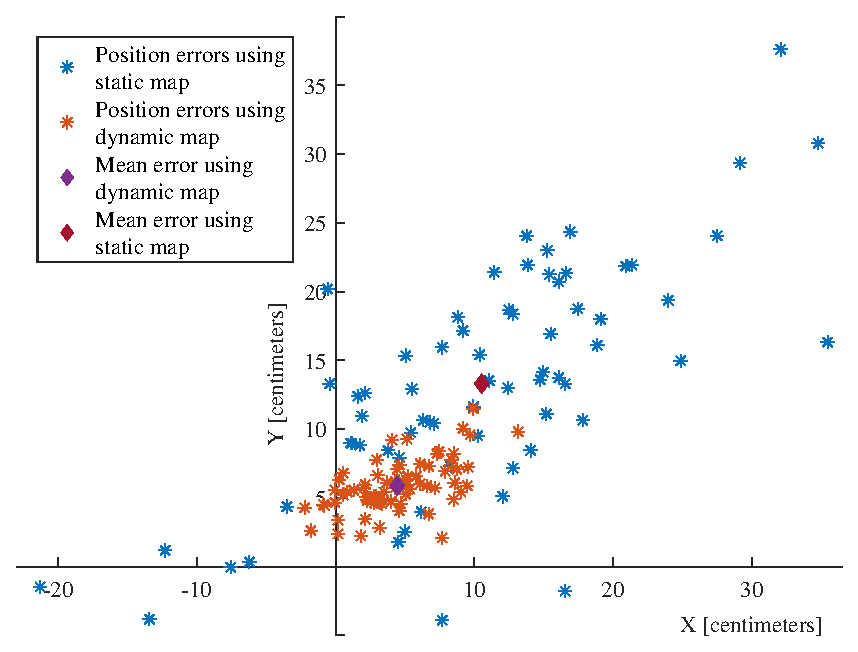
\includegraphics[scale=1]{chapters/evaluation/figures/Localization_position_errors}
    \caption{Deviation in estimated robot position when using a static or dynamic map.}
    \label{fig:precision_test_positions}
\end{figure}

\begin{figure}
    \centering
    \includegraphics[scale=1]{chapters/evaluation/figures/localization_position_error_distance-crop}
    \caption{Norm2 deviation in estimated robot position when using a static or dynamic map.}
    \label{fig:localization_position_error_distance-crop}
\end{figure}

The estimated angle deviates less, as show in figure \ref{fig:precision_test_angles}. 
There is no significant difference in mean, or median, angle error, when using a dynamic map compared to a static.

The precision of the estimated angle is however significantly smaller when using a dynamic map, as shown with the one-sided F-test for equal variance, which is rejected with $p<0.001$.
The improvement amounts to $56.7\%$ lower standard deviation when using a dynamic map instead of a static.

The statistics for the localization errors when using a static and dynamic map are summarized in table \ref{tab:localization_errors}. It shows improved accuracy and precision in the position estimation when using a dynamic map. The precision is also radically improved for the orientation estimation, but there is only a small difference in the accuracy.
\begin{figure}
    \centering
    \includegraphics[scale=1]{chapters/evaluation/figures/localization_angle_error-crop}
    \caption{Deviation in estimated robot orientation when using a static or dynamic map.}
    \label{fig:precision_test_angles}
\end{figure}

\begin{table}[htbp]
    \caption{Statistics for localization errors}
    \label{tab:localization_errors}
    \begin{center}
        \begin{tabular}{l c  c  c  c}
            \toprule
            \textbf{Map type} & \textbf{Mean position} & $\boldsymbol{\sigma_{position}}$  & \textbf{Mean angle} & $\boldsymbol{\sigma_{angle}}$\\ 
            \rowcolor[gray]{0.925}
            Dynamic & $7.7cm$ & $2.9cm$ & $0.5^\circ$ & $0.9^\circ$  \\ 
            Static & $19.4cm$ & $9.7cm$ & $0.7^\circ$ & $2.2^\circ$  \\ 	
            \bottomrule
        \end{tabular} 
    \end{center}
\end{table}